\subsection{Arten von Lasern}
	Allgemein k�nnen Laser in f�nf unterschiedliche Typen unterteilt werden:
	\begin{itemize}
		
		\item Gaslaser
		\item Festk�rperlaser
		\item Diodenlaser
		\item Freie Elektronenlaser
		\item Farbstofflaser
		
	\end{itemize}
	Das Laseraktive Medium kann entweder durch das optische Pumpen (mit Licht), durch Strom oder durch einen chemischen Prozess angeregt werden.
	Es eignet sich jedoch nicht jeder Laser zur Materialverarbeitung.\cite{eval.at2024} Die in der Materialverarbeitung am verbreitensten Laser sind folgende:
	
	\subsubsection{CO2-Laser}
		Dies ist der in der Industrie am meist verbreiteste Gaslaser, andere Gaslaser z.B N2-Laser oder Excimerlaser haben eine �hnliche Funktionsweise, aber andere Eigenschafften. Durch Zufuhr von elektrischer Energie �ber Elektroden in ein Gasgemisch von ca. 70\% He, 20\% N2 und 10\% CO2 wird das Gas zun�chst in ein elektrisch leitendes Plasma verwandelt, welches anschlie�end durch eine Reihe von Spiegeln konzentriert und fokussiert wird. Da diese Laser einen Wirkungsgrad von maximal 15\% haben, sie bei hohen Leistungen eine sehr hohe Verlustleistung, die abgef�hrt werden muss. sie werden deswegen im Bereich von 10 bis 200Watt zum Schneiden und gravieren von d�nnen organischen Materialien wie Kunsstoffe, Holz oder Textilien verwendet.\cite{eval.at2024}
	
	\begin{figure}[H]
		\centering
		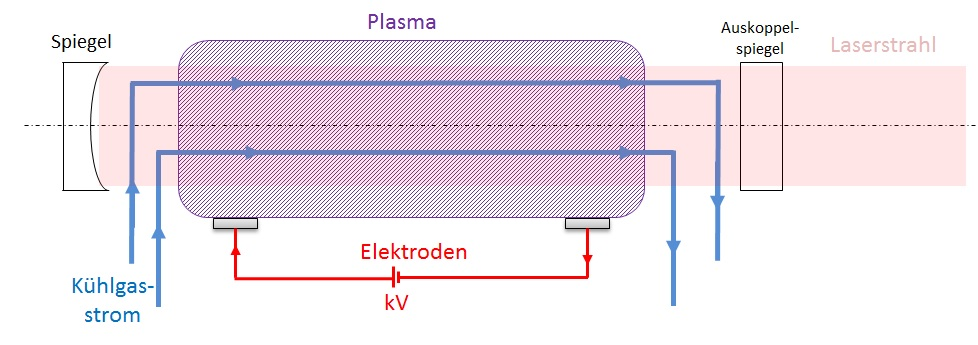
\includegraphics[scale=0.5]{./3_Stand_der_Technik/Abbildungen/Gaslaser_1}
		\caption{Aufbau eines Gaslasers\cite{eval.at2024}}
	\end{figure}
	
	\subsubsection{HeNe-Laser}
		Der HeNe Laser ist ein Gaslaser mit �hnlicher Funktionsweise zum CO2-Laser. �r wird meistens als Justierlaser verwendet, da er mit einer Leistung von unter 5mW einen sehr gut sichtbaren roten Laser erzeugt. Es sind auch andere Farben bzw Wellenl�ngen m�glich.\cite{eval.at2024}
		
	\subsubsection{Nd:YAG-Laser}
		Bei diesem Laser besteht das Lasermedium aus einem Kristall, die Energiezufuhr erfolgt durch Licht. Ein Nd:YAG-Laser(Neodym-dotierter Yttrium-Aluminium-Granat-Laser) emittiert meist eine infrarote Strahlung. Die Form dieses Kristalls ist meist in Stabform z.B. mit Durchmesser von 1cm und einer L�nge von 10cm. Er wird zwichen zwei Spiegeln positioniert und durch Blitzlampen oder Laserdionden angepumpt. Der mit Blitzlampen angepumpte Nd:YAG Laser is weiterhin der am meist verbreitete Festk�rperlaser. Ein gro�er Vorteil dieses Lasers ist auch, dass er sich im Gegensatz zum CO2-Laser durch eine Glasfa�er leiten l�sst und so f�r den Einsatz auf Roboterarmen geeignet ist.\cite{eval.at2024}
		
		\begin{figure}[H]
			\centering
			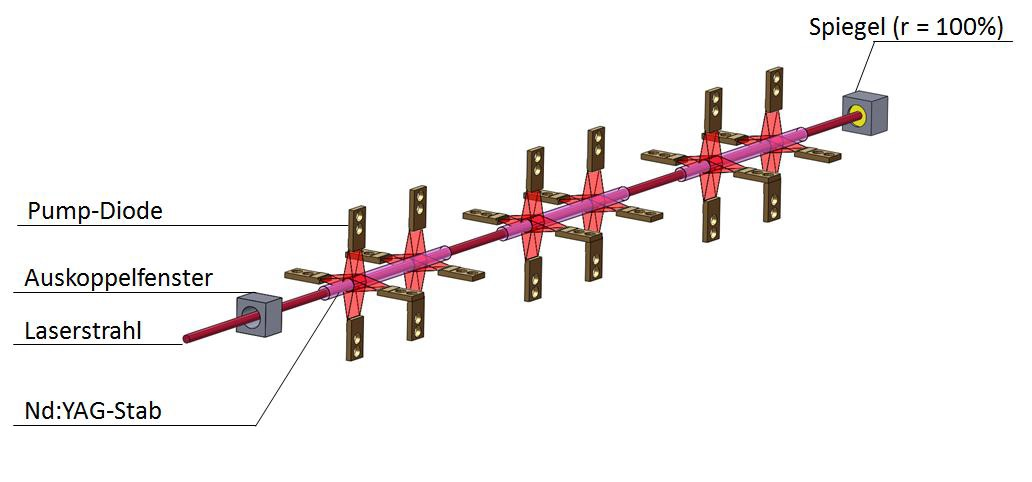
\includegraphics[scale=0.5]{./3_Stand_der_Technik/Abbildungen/NdYAGlaser_1}
			\caption{Aufbau eines Nd:YAG-Lasers\cite{eval.at2024}}
		\end{figure}
		
	\subsubsection{Faserlaser}
		Der Faserlaser besteht aus mehreren Metern lichtleitenden Faser, die mit laseraktiven Atomen dotiert sind. Durch den geringen Durchmeser dieser,(<100micrometer) erzeugt er nur Licht h�chster Strahlqualit�t und erreicht eine Effizienz von bis zu 30\%.\cite{eval.at2024}
		
	\subsubsection{Diodenlaser}
		Der Diodenlaser funktionier aufgrund vom Prinzip des pn-�bergangs von Halbleitern. Er hat eine sehr kompakte Bauweise und einen sehr hohen Wirkungsgrad von bis zu 50\%. Er besitzt im Vergleich zu anderen Lasern jedoch schlechter Strahlenqualit�t und eignet sich so eher nicht zum Schneiden.\cite{eval.at2024}
		
		\begin{figure}[H]
			\centering
			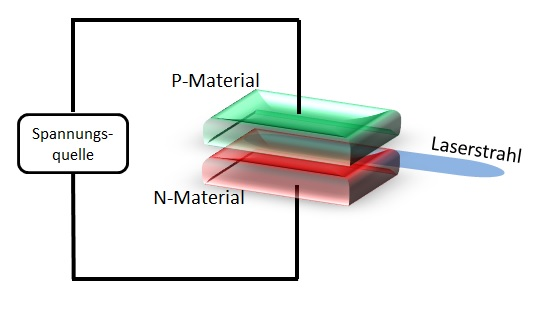
\includegraphics[scale=0.5]{./3_Stand_der_Technik/Abbildungen/Diodenlaser_1}
			\caption{Aufbau eines Diodenlasers\cite{eval.at2024}}
		\end{figure}